\documentclass[utf8]{article}
\usepackage{amsmath,amssymb}
\usepackage{graphicx}
\usepackage{fullpage}
\usepackage{setspace}
\usepackage{verbatim}

\usepackage{algorithm}
\usepackage{algorithm}
\usepackage{algorithmicx}
\usepackage{algpseudocode}
\usepackage{amsmath}
\usepackage[top=2cm, bottom=2cm, left=2cm, right=2cm]{geometry}

\onehalfspacing

\title{\bf\huge Ray Tracing Renderer}
\author{Mei Yixuan}
\date{\today}

\begin{document}
\maketitle

\section{Introduction}
This document describes the design of a simple ray tracing renderer, along with some sample scenes rendered using it. I finished it as course project for Advanced Computer Graphics, given by Prof. Shimming Hu in Tsinghua University.

Complete code for this renderer can be found in https://github.com/AntonyMei/RayTracingRender, along with all external libraries and resources. This code is designed for this course project only and implies no warranty, use at your own risk. All code follow Apache License 2.0, except those external libraries and resources.

\section{Results}
This sections shows some of the demo scenes rendered using this renderer.

\subsection{Hollow Glass Ball}
\begin{figure}[H]
	\centering
	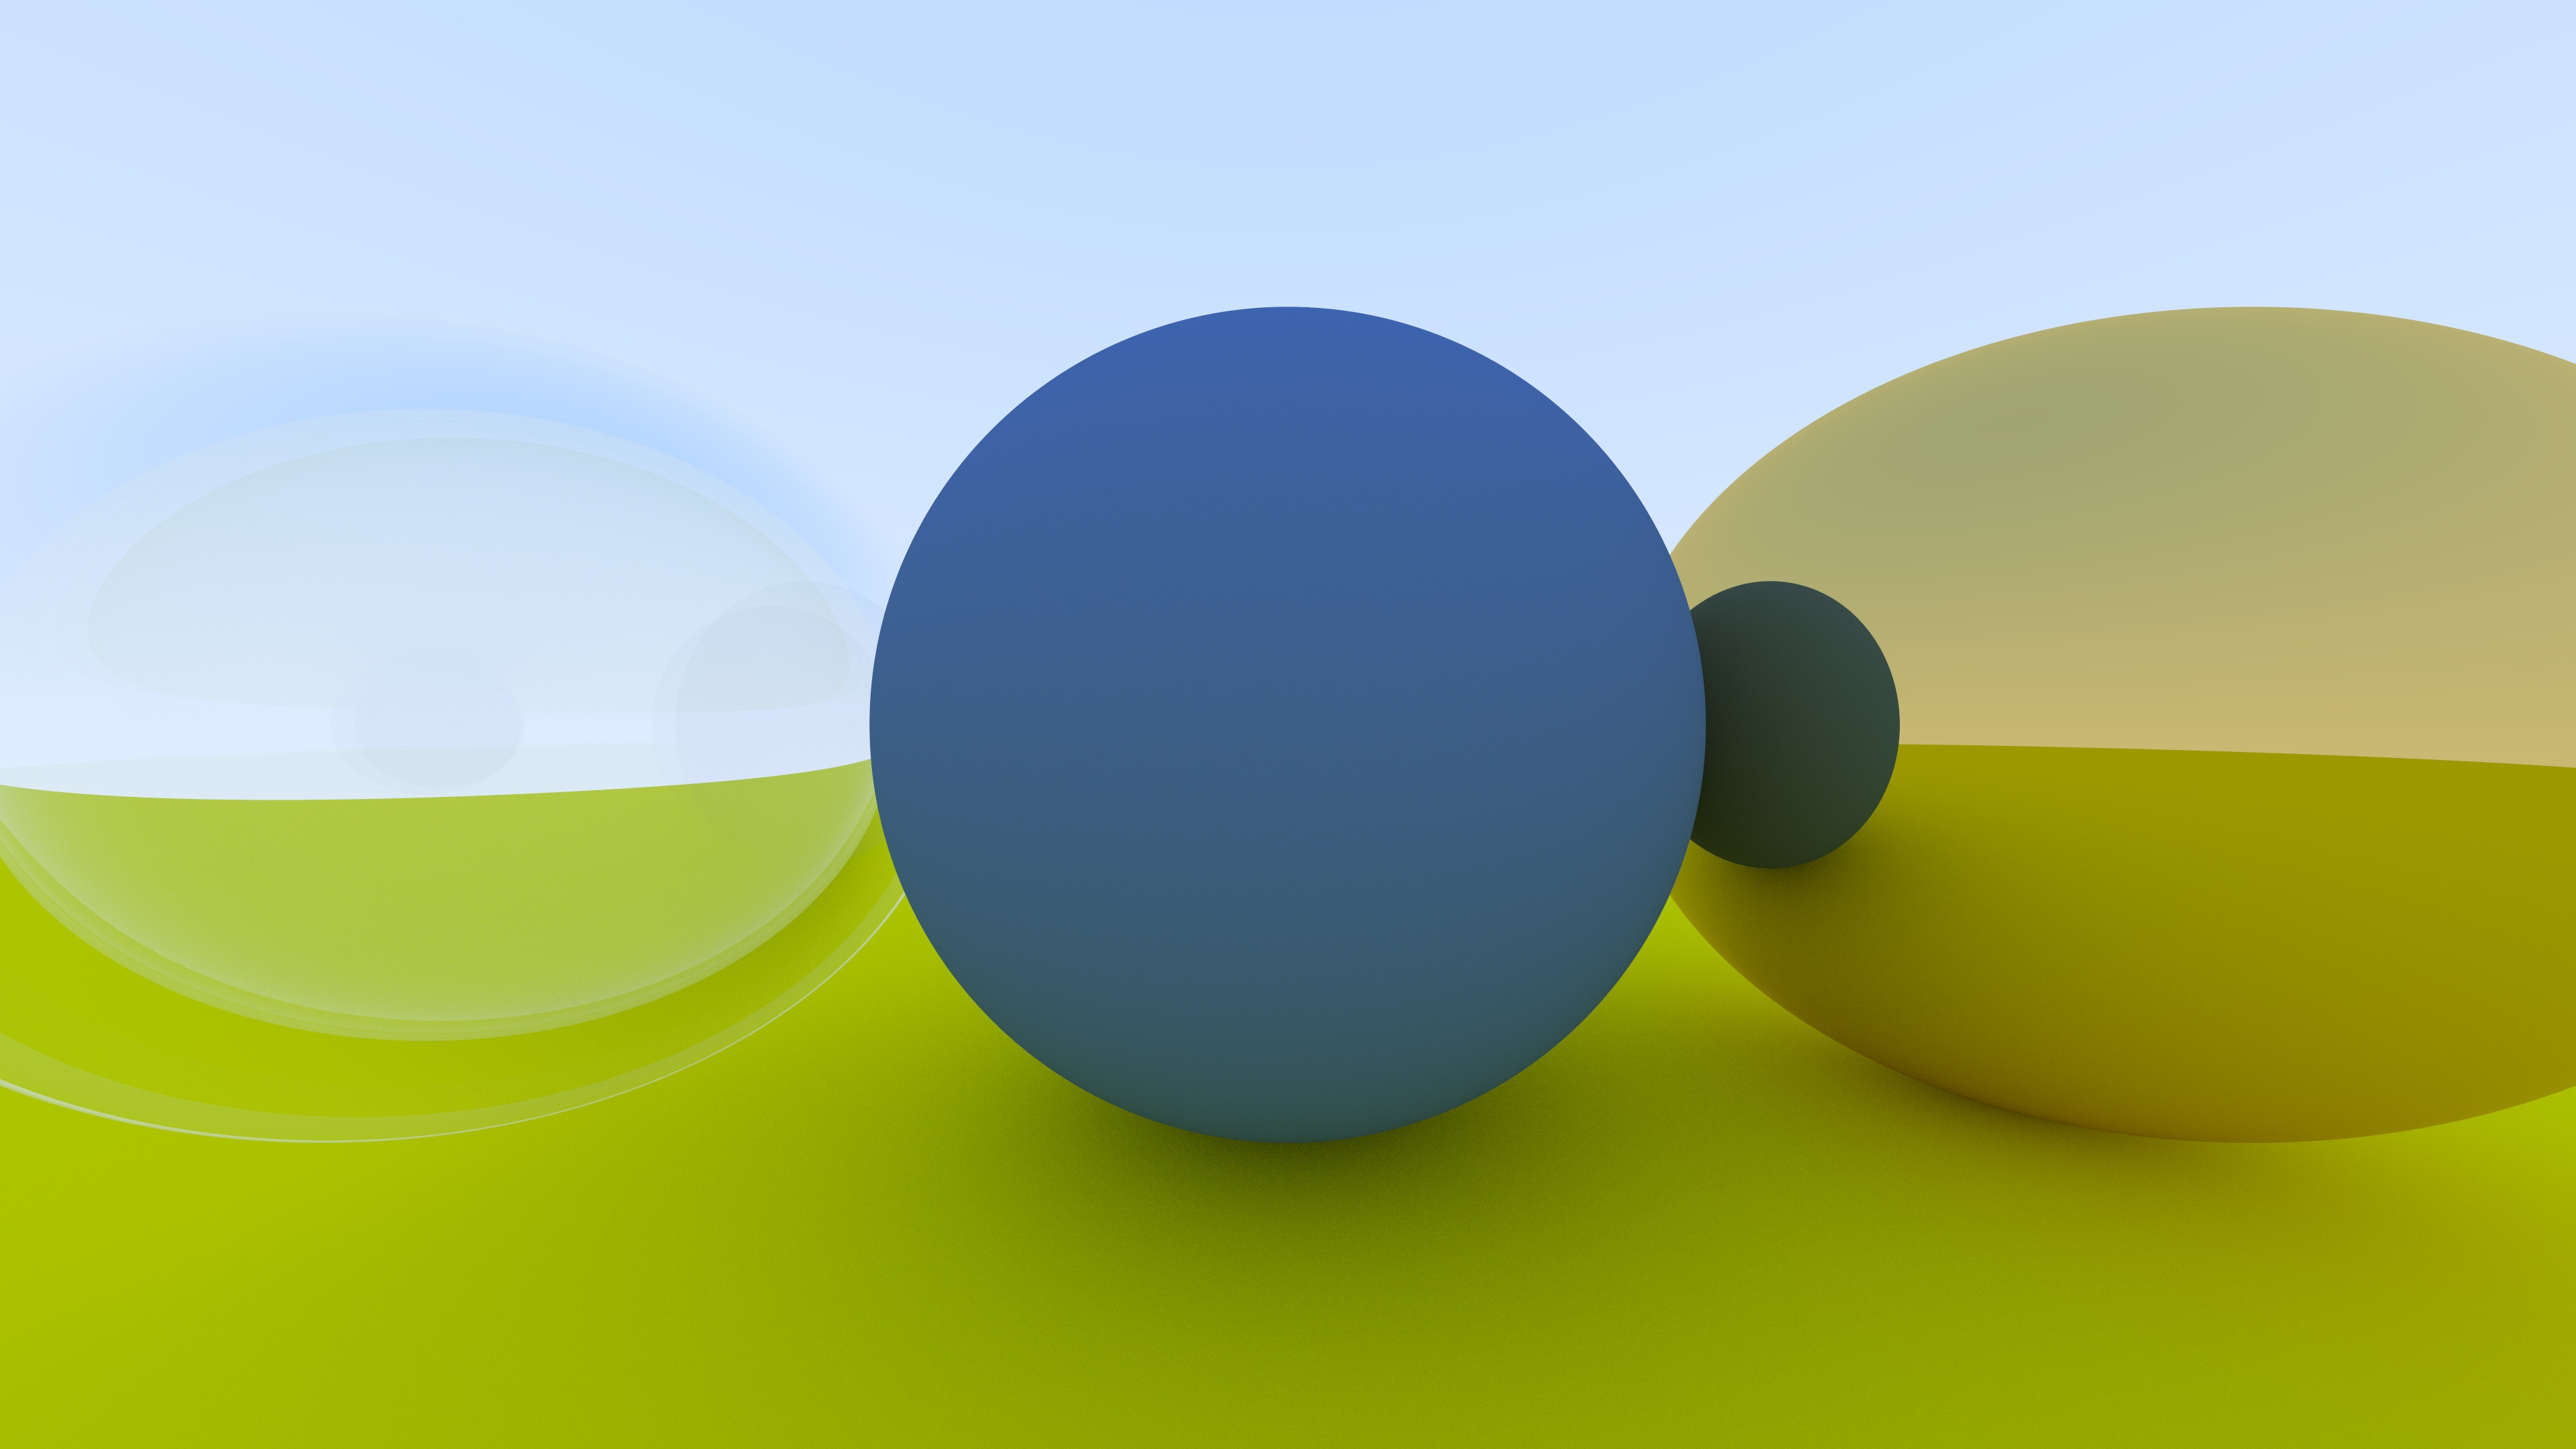
\includegraphics[width=0.7\linewidth]{../_results/hollow_glass_ball}
	\caption{Hollow Glass Ball}
	\label{fig:hollowglassball}
\end{figure}
This scene shows the usage of Lambertian (pure diffuse), Metallic (pure reflection) and Dielectric (refraction with full reflection) material

\section{Usage}

\section{Renderer Structure}
The basic structure of this renderer is as follows:

\subsection{Basic Renderer:}
\noindent
\textbf{Integrator: } Monte Carlo Path Tracing, Photon Mapping.

\noindent
\textbf{Accelerator: } BVH (AABB with SAH), Kd-Tree.

\noindent
\textbf{Hardware Acceleration: } OpenMP on Windows, Multi-processing on Linux.

\subsection{Objects: }
\noindent
\textbf{Hittable Objects: } Triangle, Triangular Mesh, Box, Sphere.

\noindent
\textbf{Complex Models: } .obj Model with .mtl Material Description.

\noindent
\textbf{Skybox: } Constant Skybox, Directional Skybox, Realistic Skybox, Multi-layer Skybox.

\noindent
\textbf{Transforms: } Rotation, Translation.

\subsection{Materials \& Textures}
\noindent
\textbf{Materials: } Lambertian, Metal, Dielectric, PBR material, Isotropic, Diffuse Light.

\noindent
\textbf{Textures: } Color Texture, Checker Texture, Perlin Noise Texture, Marble Texture, Image Texture, Bump Texture.

\subsection{Visual Effects}
\noindent
\textbf{Camera Effects: } Off-focus Blur, Motion Blur.

\noindent
\textbf{Volumetric Rendering: } Participating Media.

\noindent
\textbf{Other Visual Effects: } Gamma Correction, Caustic.

\section{Code Explanation}

\section{References}
\noindent
\textbf{Code References: }

\noindent
\textbf{[1]} Ray Tracing Mini-books, by Peter Shirley (https://raytracing.github.io)

\noindent
\textbf{[2]} Physically Based Rendering: From Theory to Implementation, by Matt Pharr, Wenzel Jakob, and Greg Humphreys (https://github.com/mmp/pbrt-v3)

\noindent
\textbf{[3]} Dezeming Family (https://dezeming.top/)

\noindent
\textbf{External Libraries: }

\noindent
\textbf{[1]} Tinyobjloader (https://github.com/tinyobjloader/tinyobjloader)

\noindent
\textbf{[2]} stb$\_$image (https://github.com/nothings/stb)

\noindent
\textbf{Model Resources: }

\noindent
\textbf{[1]} Morgan McGuire, Computer Graphics Archive, July 2017 (https://casual-effects.com/data)

\end{document}